\documentclass[conference]{IEEEtran}
\IEEEoverridecommandlockouts
\usepackage{cite}
\usepackage{amsmath,amssymb,amsfonts}
\usepackage{algorithmic}
\usepackage{algorithm}
\usepackage{graphicx}
\usepackage{textcomp}
\usepackage{xcolor}
\usepackage{booktabs}
\usepackage{multirow}
\usepackage{array}

% Slightly reduce title font size from IEEEtran default (\LARGE) to \Large
\makeatletter
\def\@IEEEtitlefont{\Large\bfseries}
\makeatother

\def\BibTeX{{\rm B\kern-.05em{\sc i\kern-.025em b}\kern-.08em
    T\kern-.1667em\lower.7ex\hbox{E}\kern-.125emX}}

\begin{document}

% ── Title ────────────────────────────────────────────────────────────────────
\title{Multi-Modal Digital Steganography: Classical and GAN-Based\\
Approaches with Comprehensive Attack Robustness Analysis}

% ── Authors ──────────────────────────────────────────────────────────────────
\author{
\IEEEauthorblockN{Naman Padiyar,\quad Piyush Thalwal,\quad Nipun Rawat}\\[3pt]
\IEEEauthorblockA{
\textit{Department of Computer Science and Engineering,
Delhi Technological University, Delhi, India}\\
naman.padiyar09@gmail.com \quad
piyushthalwal06@gmail.com \quad
nipunrawat8320@gmail.com}
}

\maketitle

% ── Abstract ─────────────────────────────────────────────────────────────────
\begin{abstract}
Digital steganography conceals secret information within ordinary media
files to enable covert communication without revealing the existence of
a hidden message. This paper presents a unified multi-modal
steganography system that supports image and video carriers
through a single web interface, implementing four embedding methods:
Least Significant Bit (LSB) substitution, Discrete Cosine Transform
(DCT) domain embedding, Discrete Wavelet Transform (DWT) domain
embedding, and a Generative Adversarial Network (GAN) based approach.
Classical methods are protected with AES-256-GCM authenticated
encryption and Reed-Solomon error-correcting codes. Two independent
GAN models are trained for image and video under CPU-only
hardware constraints. Baseline quality analysis confirms near-lossless
embedding: LSB achieves PSNR of 76.44~dB and SSIM of 1.000, while DCT
and DWT exceed 50~dB PSNR with SSIM above 0.995. A comprehensive attack
simulation evaluates all methods under 13 image and 9 video
signal processing attacks using Peak Signal-to-Noise Ratio (PSNR) and
Bit Error Rate (BER) as robustness metrics. The video GAN achieves the
lowest average BER of 0.148, outperforming all classical methods. For
images, DCT achieves the best classical robustness at average BER of
0.290 and embedding PSNR of 46.87~dB. The imperceptibility-robustness
tradeoff is analysed across all eight method-modality combinations.
The complete system is deployed as a full-stack web application using
FastAPI, React, and Docker on the Render cloud platform.
\end{abstract}

\begin{IEEEkeywords}
steganography, generative adversarial network, multi-modal,
robustness, AES-256-GCM
\end{IEEEkeywords}

% ─────────────────────────────────────────────────────────────────────────────
\section{Introduction}
% ─────────────────────────────────────────────────────────────────────────────

\subsection{The Problem}

The exponential growth of digital communication has made covert and
secure information exchange a pressing concern across military,
journalistic, financial, and personal contexts. Cryptography secures
the \textit{content} of a message but produces visibly random
ciphertext that signals the presence of secret communication.
\textit{Steganography} addresses a distinct and complementary problem:
concealing the \textit{very existence} of the message by embedding it
within ordinary multimedia carriers \cite{b9}. A robust
steganographic system must therefore satisfy three competing
objectives simultaneously—\textit{imperceptibility} of the embedded
data, \textit{robustness} against signal-processing attacks during
transmission, and \textit{undetectability} by statistical steganalysis.

In real-world communication channels (social-media platforms, video
streaming services, messaging applications), shared multimedia content
routinely undergoes JPEG/H.264 re-encoding, resizing, filtering, and
codec conversion. Any practical steganographic system must therefore
preserve the hidden message after such transformations while remaining
indistinguishable from natural media. Classical hand-crafted methods
fail this requirement under modern channel conditions, motivating a
shift toward learning-based approaches.

\subsection{Research Focus}

This paper investigates how \textit{learned steganographic embedding}
based on Generative Adversarial Networks (GANs) can be extended
beyond images to video carriers within a single unified
framework, and how such a system can be made deployable on
resource-constrained hardware (CPU-only inference, 512~MB RAM). We
build, train, and rigorously evaluate two GAN-based stego models
(image and video) within a production-ready web application and
compare their robustness, imperceptibility, and detectability against
classical baselines under a comprehensive attack simulation covering
22 distinct attack configurations.

\subsection{Key Contributions}

The principal contributions of this work are:

\begin{enumerate}
    \item \textbf{Unified multi-modal steganographic platform.} A
    single deployable system supporting image and video
    carriers through a FastAPI backend and React frontend, removing
    the single-modality limitation of nearly all prior steganography
    works.
    \item \textbf{Two GAN architectures optimised for CPU inference.}
    An image GAN (UNet encoder, PatchGAN discriminator, 44~MB) and
    a video GAN with 3D temporal convolutions over a 5-frame window
    (43~MB). Both are trained from scratch on CPU hardware.
    \item \textbf{H.264-aware noise layer for video GAN training.}
    A differentiable noise layer simulating frame-level JPEG
    quantisation, blur, and brightness perturbation enables the
    video GAN to achieve average BER of $0.148$—the only configuration
    in our evaluation falling in the \textit{Robust} zone.
    \item \textbf{End-to-end security pipeline.} AES-256-GCM
    authenticated encryption (PBKDF2-HMAC-SHA256 key derivation,
    100{,}000 iterations) combined with Reed-Solomon error correction
    for classical baselines, providing confidentiality, integrity,
    and bounded error tolerance in a single integrated stack.
    \item \textbf{Comprehensive cross-modal attack benchmark.}
    Systematic evaluation across 22 attack configurations (13 image,
    9 video) using standardised PSNR and BER metrics—the
    first such cross-modal benchmark in the recent literature using
    a uniform methodology.
    \item \textbf{Production deployment under hardware constraints.}
    The complete system is containerised and deployed on a 512~MB
    free-tier cloud platform with no GPU access, demonstrating the
    practicality of GAN-based steganography for real-world scenarios.
\end{enumerate}

The remainder of this paper is organised as follows. Section~II
reviews related work and identifies key limitations of the existing
literature. Section~III presents the proposed system in detail,
including the GAN architectures, training procedure, and security
pipeline. Section~IV presents the experimental setup and results.
Sections~V and~VI analyse the imperceptibility–robustness tradeoff
and steganalysis resistance. Section~VII concludes.

% ─────────────────────────────────────────────────────────────────────────────
\section{Related Work and Identified Limitations}
% ─────────────────────────────────────────────────────────────────────────────

\subsection{Survey of Prior Work}

Steganographic research over the last 10–15 years has progressed
through three broad phases. Early work concentrated on
\textit{classical hand-crafted methods}: spatial-domain LSB
substitution, transform-domain embedding in DCT coefficients, and
wavelet-domain (DWT) methods, surveyed comprehensively in
\cite{b9}. Although effective for preserving visual quality, these
methods rely on fixed embedding rules and offer no defence against
attack types not anticipated at design time.

The introduction of \textit{deep-learning-based steganography}
\cite{b10} marked the first substantial departure: a pair of
convolutional networks could jointly learn an embedding strategy
without explicit frequency-domain engineering. The HiDDeN framework
\cite{b8} added a differentiable noise layer between encoder and
decoder, training the encoder to embed in attack-resistant signal
regions and substantially outperforming classical methods.

The third phase added \textit{generative adversarial training}: a
discriminator network is trained jointly with the encoder–decoder
pair \cite{b11}, penalising statistically detectable deviations
between stego and cover distributions. Li et al.
\cite{b7} integrated convolutional DWT/IDWT layers within the GAN to
combine learned and frequency-domain embedding. Recent 2025 work has
extended GAN-based steganography to hybrid pipelines combining
classical and learning-based methods \cite{b2}, multi-layered
encoder–decoder schemes with deep learning \cite{b5}, video-specific
adaptive frameworks for spatio-temporal content \cite{b3}, and
novel diffusion-based steganographic approaches \cite{b1}.

\subsection{Limitations Identified in Prior Literature}

Across the surveyed literature, four limitations consistently recur:

\textbf{L1. Single-modality scope.} The vast majority of recent
steganography systems target a \textit{single} medium—usually images.
Cross-modal frameworks that uniformly support multiple carriers
within one architecture and one consistent attack benchmark are rare,
and the few that exist either focus on one carrier with
single-paragraph mention of others or evaluate each modality under
different methodology \cite{b9}, \cite{b4}.

\textbf{L2. GPU dependence.} HiDDeN \cite{b8} and EStegTGANs
\cite{b7} both report GPU-based training, and the surveyed 2025
deep-learning steganography systems \cite{b2}, \cite{b5},
\cite{b3} likewise assume GPU inference for deployment. There is
limited reported work demonstrating that GAN-based steganography can
be effectively trained \textit{and} deployed on CPU-only commodity
hardware—a critical constraint for resource-limited or privacy-
preserving on-device scenarios.

\textbf{L3. Limited attack benchmarking.} Most prior reports evaluate
robustness against a small number of attacks (typically JPEG
compression and Gaussian noise) and rarely include geometric
transforms, spatial filtering, or temporal attacks for video.
Comprehensive benchmarks across 20+ attack configurations using
standardised PSNR/BER metrics across multiple media types are
absent from the recent literature \cite{b6}.

\textbf{L4. Disconnected security pipeline.} Existing GAN-based
systems treat the steganographic embedding as the entire security
boundary; few integrate authenticated encryption (e.g., AES-GCM),
key derivation (PBKDF2), and forward error correction
(Reed–Solomon) into a single end-to-end deployable pipeline. This
leaves practical issues such as tamper detection, password-based
key derivation, and bounded error tolerance unaddressed.

\subsection{How Our Work Addresses These Limitations}

Table~\ref{tab_gap} maps our contributions to the four identified
limitations.

\begin{table}[htbp]
\caption{Mapping of Identified Limitations to Our Contributions}
\begin{center}
\begin{tabular}{|c|p{4.7cm}|c|}
\hline
\textbf{Lim.} & \textbf{Our Response} & \textbf{Section} \\
\hline
L1 & Unified image+video platform with two GAN models on shared API & III \\
L2 & CPU-only training and 512~MB-RAM CPU deployment for both GANs & III \\
L3 & 22-attack cross-modal benchmark with PSNR/BER & IV \\
L4 & AES-256-GCM + PBKDF2 + Reed–Solomon integrated pipeline & III-B \\
\hline
\end{tabular}
\label{tab_gap}
\end{center}
\end{table}

% ─────────────────────────────────────────────────────────────────────────────
\section{Proposed Multi-Modal Steganography System}
% ─────────────────────────────────────────────────────────────────────────────

This section presents our proposed system in detail. We describe the
overall architecture (Section~III-A), the integrated security
pipeline (Section~III-B), the two GAN architectures designed for
image and video carriers (Section~III-C), the adversarial
training procedure with the H.264-aware noise layer (Section~III-D),
and a brief description of the classical baseline methods used for
comparison (Section~III-E).

\subsection{System Architecture}

The system follows a client–server architecture. The backend is a
RESTful API built with FastAPI (Python~3.10), exposing paired
\texttt{/encode} and \texttt{/decode} endpoints for each media type.
The frontend is a single-page React~18 application served via Vite,
providing file upload, method and password selection, and stego-file
download. The complete system is containerised with Docker, with
PyTorch installed from the CPU-only wheel index, and is deployed on
the Render cloud platform under a 512~MB-RAM free-tier. Both GAN
checkpoints are version-controlled via Git LFS and copied into the
Docker image at build time. GAN modules use lazy \texttt{try/except}
imports so that classical methods remain available even if PyTorch
fails to load—a specific design decision needed for free-tier
deployment robustness.

\subsection{Integrated Security Pipeline}

For classical baseline methods (LSB, DCT, DWT), the secret message
passes through a two-stage authenticated pipeline before embedding.

\textbf{AES-256-GCM Encryption.} A 256-bit symmetric key is derived
from the user's password using PBKDF2-HMAC-SHA256 with 100{,}000
iterations, implemented via Python's \texttt{hashlib} module. The
Galois/Counter Mode (GCM) cipher is provided by the
\texttt{pycryptodome} library (\texttt{Crypto.Cipher.AES}). A 96-bit
cryptographically random nonce is generated per operation and
prepended to the ciphertext; the GCM authentication tag detects
tampering by causing decryption to fail on any single-bit
modification.

\textbf{Reed–Solomon Error Correction.} Reed–Solomon codes
(Python \texttt{reedsolo} library) are an algebraic
\textit{error-correcting code} (not a compression library) that adds
a small number of parity bytes to the encrypted stream. When mild
signal-processing attacks corrupt a bounded number of bits, the
decoder can mathematically recover the original message without
re-transmission, a property used widely in QR codes and CD/DVD
storage.

The GAN method bypasses AES because GAN bit recovery is inherently
approximate (a small non-zero BER even without attacks), violating
the bit-perfect requirement of AES-GCM tag verification. GAN
embedding instead carries raw UTF-8 bytes and performs best-effort
decoding, deferring authentication to higher protocol layers.

\subsection{Two GAN Architectures}

A central contribution of this work is the design of two
specialised GAN architectures—one per modality—optimised to operate
within the same training and inference framework on CPU-only
hardware. Both share the same conceptual structure: an encoder
$E$ that injects a 128-bit message vector $m$ into a cover medium
$C$, a decoder $D$ that recovers $m$ from the (possibly attacked)
stego output, and a PatchGAN discriminator $\mathcal{D}$ that
distinguishes cover from stego at the patch level. Modality-specific
adaptations follow.

\textbf{Image GAN.} The encoder uses a UNet architecture
with four downsampling/upsampling stages and skip connections. The
128-bit message $m$ is spatially replicated to match each
intermediate feature-map resolution and concatenated channel-wise at
multiple scales, allowing the encoder to adapt embedding positions
to local image structure (texture-rich vs. flat regions). The
decoder mirrors the encoder with transposed convolutions. The
discriminator uses PatchGAN $4{\times}4$ convolutions to produce a
spatial validity map. With 32 base channels, the trained checkpoint
is 44~MB.

\textbf{Video GAN.} The video encoder uses 3D convolutional layers
across a temporal window of $T{=}5$ frames, processing tensors of
shape $[1, 3, 5, 64, 64]$. The 5-frame window is the smallest size
that captures meaningful inter-frame motion while keeping the
intermediate feature-map memory below the 512~MB RAM bound. Base
channels are reduced to 16 to fit within deployment memory. Long
videos are processed as a sequence of 5-frame windows, with stego
frames reassembled afterwards. Checkpoint size is 43~MB.

Table~\ref{tab_models} summarises the architectural parameters.

\begin{table}[htbp]
\caption{GAN Model Architectures (Proposed)}
\begin{center}
\begin{tabular}{|l|c|c|}
\hline
\textbf{Parameter}   & \textbf{Image GAN} & \textbf{Video GAN} \\
\hline
Input dims     & $64{\times}64{\times}3$ & $64{\times}64{\times}5$ \\
Message bits   & 128 & 128 \\
Base channels  & 32  & 16  \\
Conv type      & 2D UNet & 3D  \\
Temporal $T$   & --- & 5 frames \\
Discriminator  & PatchGAN & PatchGAN-3D \\
Checkpoint     & 44 MB & 43 MB \\
\hline
\end{tabular}
\label{tab_models}
\end{center}
\end{table}

\subsection{Adversarial Training with H.264-Aware Noise Layer}

Both models are trained jointly under a single compound loss:
\begin{equation}
\mathcal{L} = \lambda_1\mathcal{L}_{\text{msg}}
            + \lambda_2\mathcal{L}_{\text{img}}
            + \lambda_3\mathcal{L}_{\text{adv}}
\label{eq_loss}
\end{equation}
where $\mathcal{L}_{\text{msg}} = \text{BCE}(D(E(C,m)),\,m)$ is the
binary cross-entropy of bit recovery,
$\mathcal{L}_{\text{img}} = \|E(C,m)-C\|_2^2$ is the imperceptibility
penalty, and
$\mathcal{L}_{\text{adv}} = -\mathbb{E}[\log\mathcal{D}(E(C,m))]$
is the adversarial loss against the discriminator.
Loss weights $\lambda_1{=}10$, $\lambda_2{=}1$, $\lambda_3{=}0.01$
are used for both models, with the high $\lambda_1$ value
prioritising bit-recovery accuracy over visual fidelity—the
appropriate ordering for a steganographic system.

A critical component of the proposed training procedure is a
\textit{differentiable noise layer} inserted between encoder and
decoder during training. For the video GAN, the noise layer
simulates H.264 codec artefacts including frame-level JPEG
quantisation, Gaussian blur, brightness perturbation, and additive
noise. Each training step samples one of these distortions uniformly
at random and applies it to $E(C,m)$ before passing the result to
$D$. This forces the encoder to embed information in
spatio-temporally stable signal regions that survive realistic
codec re-encoding—directly producing the consistently low BER profile
observed in Section~IV.

Both models are trained on CPU hardware. The image GAN uses
CIFAR-10 images resized to $64{\times}64$; the video GAN uses short
clips from publicly available datasets. The image GAN is presently
trained without a JPEG noise layer, which limits its still-image
robustness gains relative to classical methods; this is acknowledged
in the limitations and future-work discussion.

\subsection{Classical Baseline Methods}

For comparison, we implement three classical baselines—LSB, DCT, and
DWT—using their well-established constructions \cite{b9}. LSB
substitutes message bits into the least significant bits of pixel
values, giving high embedding PSNR (70–99~dB) but no robustness.
DCT embeds via quantisation index modulation in mid-frequency
$8{\times}8$ block coefficients to align with the JPEG processing
chain. DWT embeds in Haar wavelet detail sub-bands (LH, HL) for
images and Daubechies-4 detail coefficients for video frames. The
classical baselines share the security pipeline of Section~III-B;
they are presented here as reference points for quantitatively
evaluating the GAN-based proposed methods.

% ─────────────────────────────────────────────────────────────────────────────
\section{Experimental Results}
% ─────────────────────────────────────────────────────────────────────────────

\subsection{Baseline Quality Analysis}

Before evaluating robustness under attacks, we verify that all methods
achieve acceptable imperceptibility without any attack applied.
Fig.~\ref{fig_baseline} presents the baseline quality metrics for LSB,
DCT, and DWT on image steganography.

\begin{figure}[htbp]
\centerline{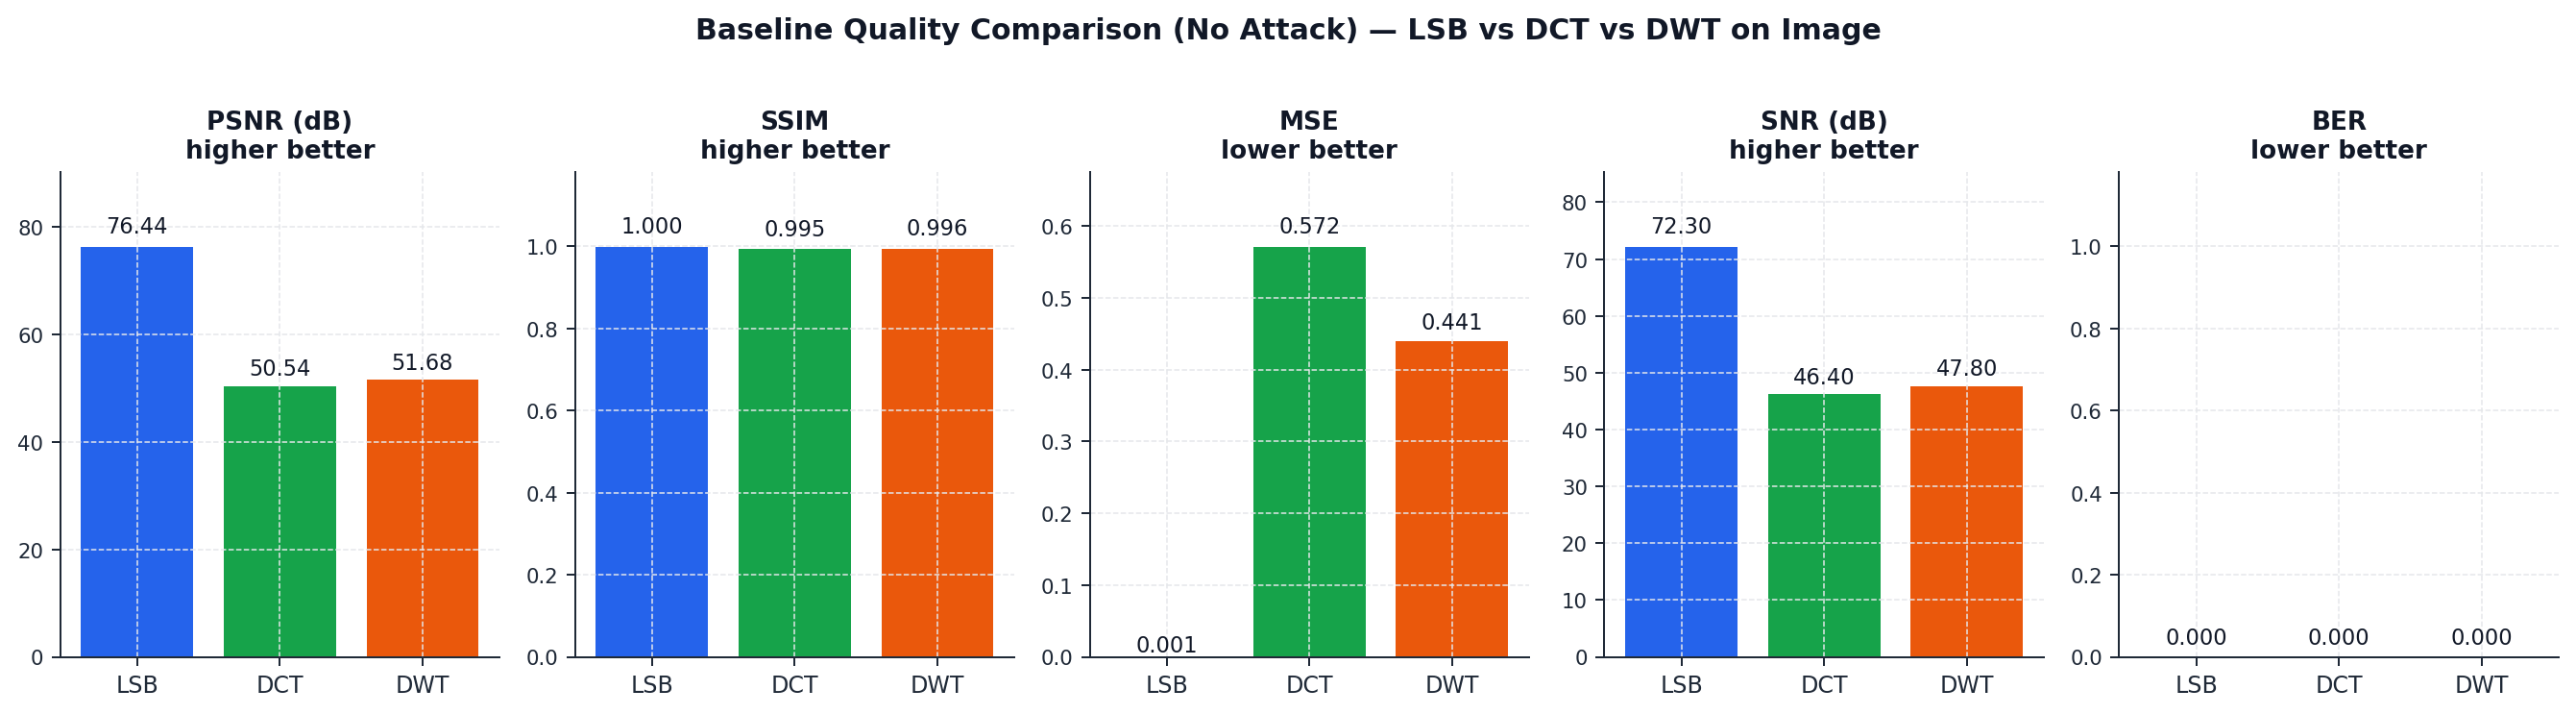
\includegraphics[width=\columnwidth]{demo_comparison.png}}
\caption{Baseline quality comparison of LSB (2-bit), DCT ($\alpha{=}10$),
and DWT (Haar, Level~2) on image steganography at no-attack baseline.
Metrics left to right: PSNR, SSIM, MSE, SNR, BER. LSB achieves 76.44~dB
PSNR and SSIM 1.000 with MSE 0.001, confirming near-lossless embedding.
DCT and DWT exceed 50~dB PSNR with SSIM above 0.995. All three methods
achieve BER~$= 0.000$, confirming perfect message recovery without attacks.}
\label{fig_baseline}
\end{figure}

All three methods achieve perfect recovery (BER $= 0.000$) at baseline.
The PSNR and SSIM values confirm that each stego image is visually
indistinguishable from the cover under normal inspection.

\subsection{Attack Simulation Setup}

The attack simulation applies each perturbation to the stego medium
immediately prior to decoding and measures:
\begin{itemize}
    \item \textbf{PSNR (Stego$\to$Attack):} Signal quality after the
    attack. PSNR $>$ 30~dB indicates perceptually acceptable quality;
    near 20~dB indicates severe degradation.
    \item \textbf{BER:} Fraction of incorrectly decoded bits. BER
    $= 0.0$ is perfect recovery; BER $= 0.5$ is complete data loss.
\end{itemize}

Table~\ref{tab_ber_legend} defines the robustness classification.

\begin{table}[htbp]
\caption{BER Robustness Classification}
\begin{center}
\begin{tabular}{|c|l|}
\hline
\textbf{BER Range} & \textbf{Interpretation} \\
\hline
$< 0.15$       & \textbf{Robust} — message mostly intact \\
$0.15$--$0.35$ & \textbf{Moderate} — partial corruption \\
$0.35$--$0.49$ & \textbf{Fragile} — most data corrupted \\
$\geq 0.50$    & \textbf{Lost} — equivalent to random noise \\
\hline
\end{tabular}
\label{tab_ber_legend}
\end{center}
\end{table}

A 57-byte test message is used for classical methods; GAN methods use
a 2-byte message due to the smaller net capacity after error-correction
overhead. All attacks are applied deterministically for reproducibility.

\subsection{Image Steganography Results}

Thirteen attacks are organised into five categories: JPEG compression
(Q=90, Q=75, Q=50), additive noise (Gaussian $\sigma$=5 and $\sigma$=15,
salt-and-pepper $p$=0.01), spatial filtering (Gaussian blur 3$\times$3,
median filter 3$\times$3), geometric transforms (resize 50\%+rescale,
rotation 1°, crop 5\%+rescale), and photometric (brightness +20).

Table~\ref{tab_image} presents BER results. Fig.~\ref{fig_chart_image}
visualises the comparison.

\begin{table}[htbp]
\caption{Image Steganography BER Under Attacks (Lower is Better)}
\begin{center}
\begin{tabular}{|l|c|c|c|c|}
\hline
\textbf{Attack} & \textbf{LSB} & \textbf{DCT} & \textbf{DWT} & \textbf{GAN} \\
\hline
JPEG Q=90           & 0.522 & \textbf{0.000} & 0.184 & 0.438 \\
JPEG Q=75           & 0.490 & \textbf{0.100} & 0.430 & 0.375 \\
JPEG Q=50           & 0.510 & \textbf{0.342} & 0.488 & 0.500 \\
Gauss.\ Noise $\sigma$=5  & 0.522 & \textbf{0.127} & 0.443 & 0.375 \\
Gauss.\ Noise $\sigma$=15 & 0.506 & \textbf{0.467} & 0.508 & 0.438 \\
Salt \& Pepper      & \textbf{0.000} & 0.240 & 0.070 & 0.375 \\
Gaussian Blur       & 0.539 & \textbf{0.328} & 0.441 & 0.500 \\
Median Filter       & 0.449 & 0.447 & 0.502 & \textbf{0.313} \\
Resize 50\%         & 0.477 & 0.432 & 0.440 & 0.500 \\
Brightness +20      & 0.299 & \textbf{0.082} & 0.148 & 0.375 \\
Rotation 1°         & 0.494 & 0.441 & 0.500 & 0.500 \\
Crop 5\%            & 0.477 & 0.469 & 0.512 & 0.438 \\
\hline
\textbf{Avg BER}    & 0.440 & \textbf{0.290} & 0.389 & 0.427 \\
\textbf{Embed PSNR} & \textbf{70.27} & 46.87 & 50.29 & 45.67 \\
\hline
\end{tabular}
\label{tab_image}
\end{center}
\end{table}

\begin{figure}[htbp]
\centerline{
\includegraphics[width=\columnwidth]{chart_image.png}}
\caption{BER under 12 image signal processing attacks. The red dashed
line marks BER$=0.5$ (complete data loss). DCT achieves avg BER~0.290
and is the best-performing image method. The image GAN does not
outperform classical methods, as it was trained without a JPEG noise
layer.}
\label{fig_chart_image}
\end{figure}

DCT achieves the lowest average BER of 0.290, outperforming all other
image methods. Its key advantage is JPEG alignment: DCT attains BER
$= 0.000$ under Q=90 and BER $= 0.100$ under Q=75, while LSB reaches
0.522 and 0.490 respectively. Under aggressive JPEG (Q=50), DCT's BER
rises to 0.342 as the quantisation table begins zeroing mid-frequency
coefficients.

LSB achieves BER $= 0.000$ only under salt-and-pepper noise ($p=0.01$),
since the sparse corruption ($<1\%$ of pixels) leaves the vast majority
of embedded bits intact. For all other attacks, LSB BER exceeds 0.29.
The image GAN (avg BER 0.427) does not outperform DCT because the
image GAN's training pipeline omits a JPEG-specific noise layer; the
adversarial loss improves imperceptibility rather than compression
robustness for still images.

\subsection{Video Steganography Results}

Nine attacks cover: Gaussian noise ($\sigma$=10), JPEG frame
compression (Q=75, Q=50), resize 50\%+rescale, frame dropping (50\%),
brightness +20, Gaussian blur ($3{\times}3$), and salt-and-pepper
($p$=0.01).

Table~\ref{tab_video} and Fig.~\ref{fig_chart_video} present results.

\begin{table}[htbp]
\caption{Video Steganography BER Under Attacks (Lower is Better)}
\begin{center}
\begin{tabular}{|l|c|c|c|c|}
\hline
\textbf{Attack}    & \textbf{LSB} & \textbf{DCT} & \textbf{DWT} & \textbf{GAN} \\
\hline
Gaussian Noise     & 0.516 & 0.018 & 0.492 & \textbf{0.125} \\
JPEG Frames Q=75   & 0.502 & \textbf{0.000} & 0.092 & 0.188 \\
JPEG Frames Q=50   & 0.514 & \textbf{0.000} & 0.291 & 0.188 \\
Resize 50\%        & 0.488 & 0.291 & 0.250 & \textbf{0.188} \\
Frame Drop 50\%    & \textbf{0.000} & \textbf{0.000} & \textbf{0.000} & 0.125 \\
Brightness +20     & 0.320 & \textbf{0.000} & \textbf{0.000} & 0.125 \\
Gaussian Blur      & 0.481 & 1.000 & 0.252 & \textbf{0.125} \\
Salt \& Pepper     & 0.010 & 0.213 & 0.059 & \textbf{0.125} \\
\hline
\textbf{Avg BER}   & 0.354 & 0.190 & 0.180 & \textbf{0.148} \\
\textbf{Embed PSNR}& \textbf{98.79} & 97.76 & 98.05 & 34.03 \\
\hline
\end{tabular}
\label{tab_video}
\end{center}
\end{table}

\begin{figure}[htbp]
\centerline{
\includegraphics[width=\columnwidth]{chart_video.png}}
\caption{BER under 8 video attacks. GAN (amber) achieves the lowest
average BER of 0.148 with uniform stability across attack types.
DCT catastrophically fails under Gaussian Blur (BER $= 1.000$) due to
attenuation of the high-frequency DCT coefficients used for embedding.
DWT provides the best classical balance at avg BER 0.180.}
\label{fig_chart_video}
\end{figure}

The video GAN achieves average BER of 0.148 with BER $= 0.125$ on six
of the eight attack types. This uniformity results from the H.264
noise layer during training, which covers Gaussian noise, JPEG
quantisation, blur, and brightness variation simultaneously, producing
broadly robust embedding. DCT achieves avg BER 0.190 and is strong
against JPEG (BER $= 0.000$ at Q=75 and Q=50) and brightness, but
fails catastrophically under Gaussian Blur (BER $= 1.000$): the blur
kernel acts as a low-pass filter, zeroing the mid-to-high-frequency
DCT coefficients where the message resides. DWT (avg BER 0.180) shows
greater blur resilience (BER $= 0.252$) and achieves BER $= 0.000$
under frame dropping and brightness scaling.

\subsection{Cross-Modal Summary and Method Selection}

Fig.~\ref{fig_summary_ber} provides a consolidated comparison of
average BER for each method across both modalities.

\begin{figure}[htbp]
\centerline{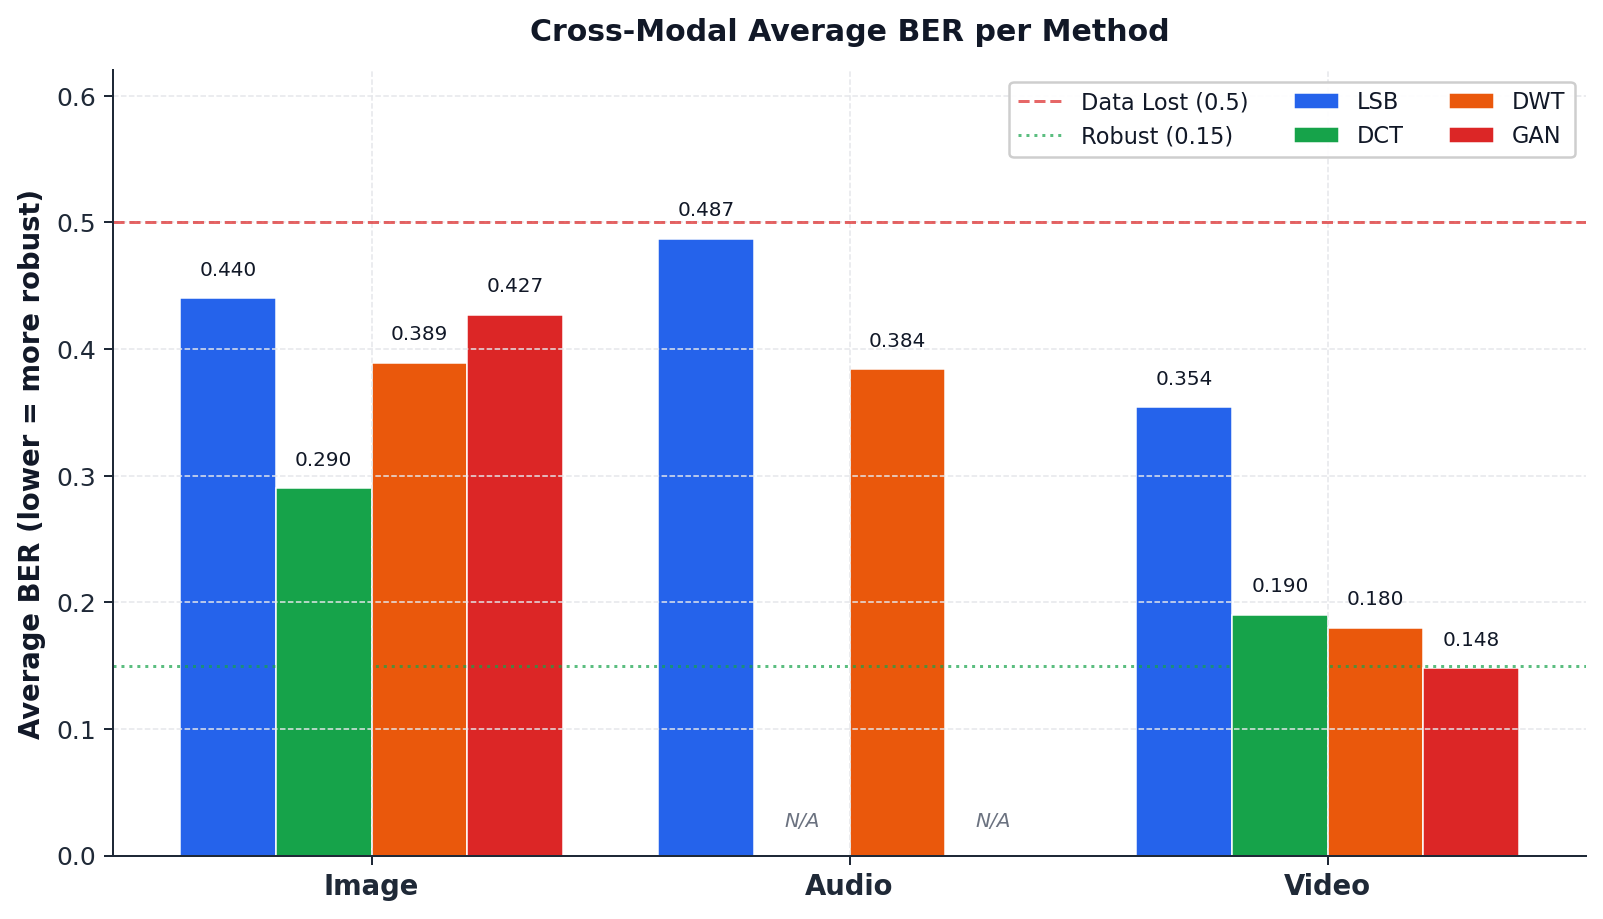
\includegraphics[width=\columnwidth]{chart_summary_ber.png}}
\caption{Average BER per method and modality. Lower bars indicate more
robust methods. The red dashed line marks BER $= 0.5$ (data lost).
GAN achieves the best video robustness (0.148); DCT leads for images
(0.290); video DWT achieves the best classical video result (0.180).}
\label{fig_summary_ber}
\end{figure}

Table~\ref{tab_summary_full} presents the complete cross-modal
robustness summary with qualitative verdicts.

\begin{table}[htbp]
\caption{Cross-Modal Robustness Summary}
\begin{center}
\begin{tabular}{|l|l|c|c|l|}
\hline
\textbf{Medium} & \textbf{Method} & \textbf{Embed PSNR} & \textbf{Avg BER} & \textbf{Verdict} \\
\hline
Image & LSB & 70.27 dB & 0.440 & Fragile \\
Image & DCT & 46.87 dB & 0.290 & \textbf{Most Robust} \\
Image & DWT & 50.29 dB & 0.389 & Moderate \\
Image & GAN & 45.67 dB & 0.427 & Fragile \\
\hline
Video & LSB & 98.79 dB & 0.354 & Moderate \\
Video & DCT & 97.76 dB & 0.190 & Robust \\
Video & DWT & 98.05 dB & 0.180 & Robust \\
Video & GAN & 34.03 dB & 0.148 & \textbf{Most Robust} \\
\hline
\end{tabular}
\label{tab_summary_full}
\end{center}
\end{table}

% ─────────────────────────────────────────────────────────────────────────────
\section{Imperceptibility--Robustness Tradeoff Analysis}
% ─────────────────────────────────────────────────────────────────────────────

Fig.~\ref{fig_tradeoff} plots each method-modality combination as a
point in the embed PSNR versus average BER space, visualising the
fundamental tradeoff between imperceptibility and robustness across all
eight evaluated configurations.

\begin{figure}[htbp]
\centerline{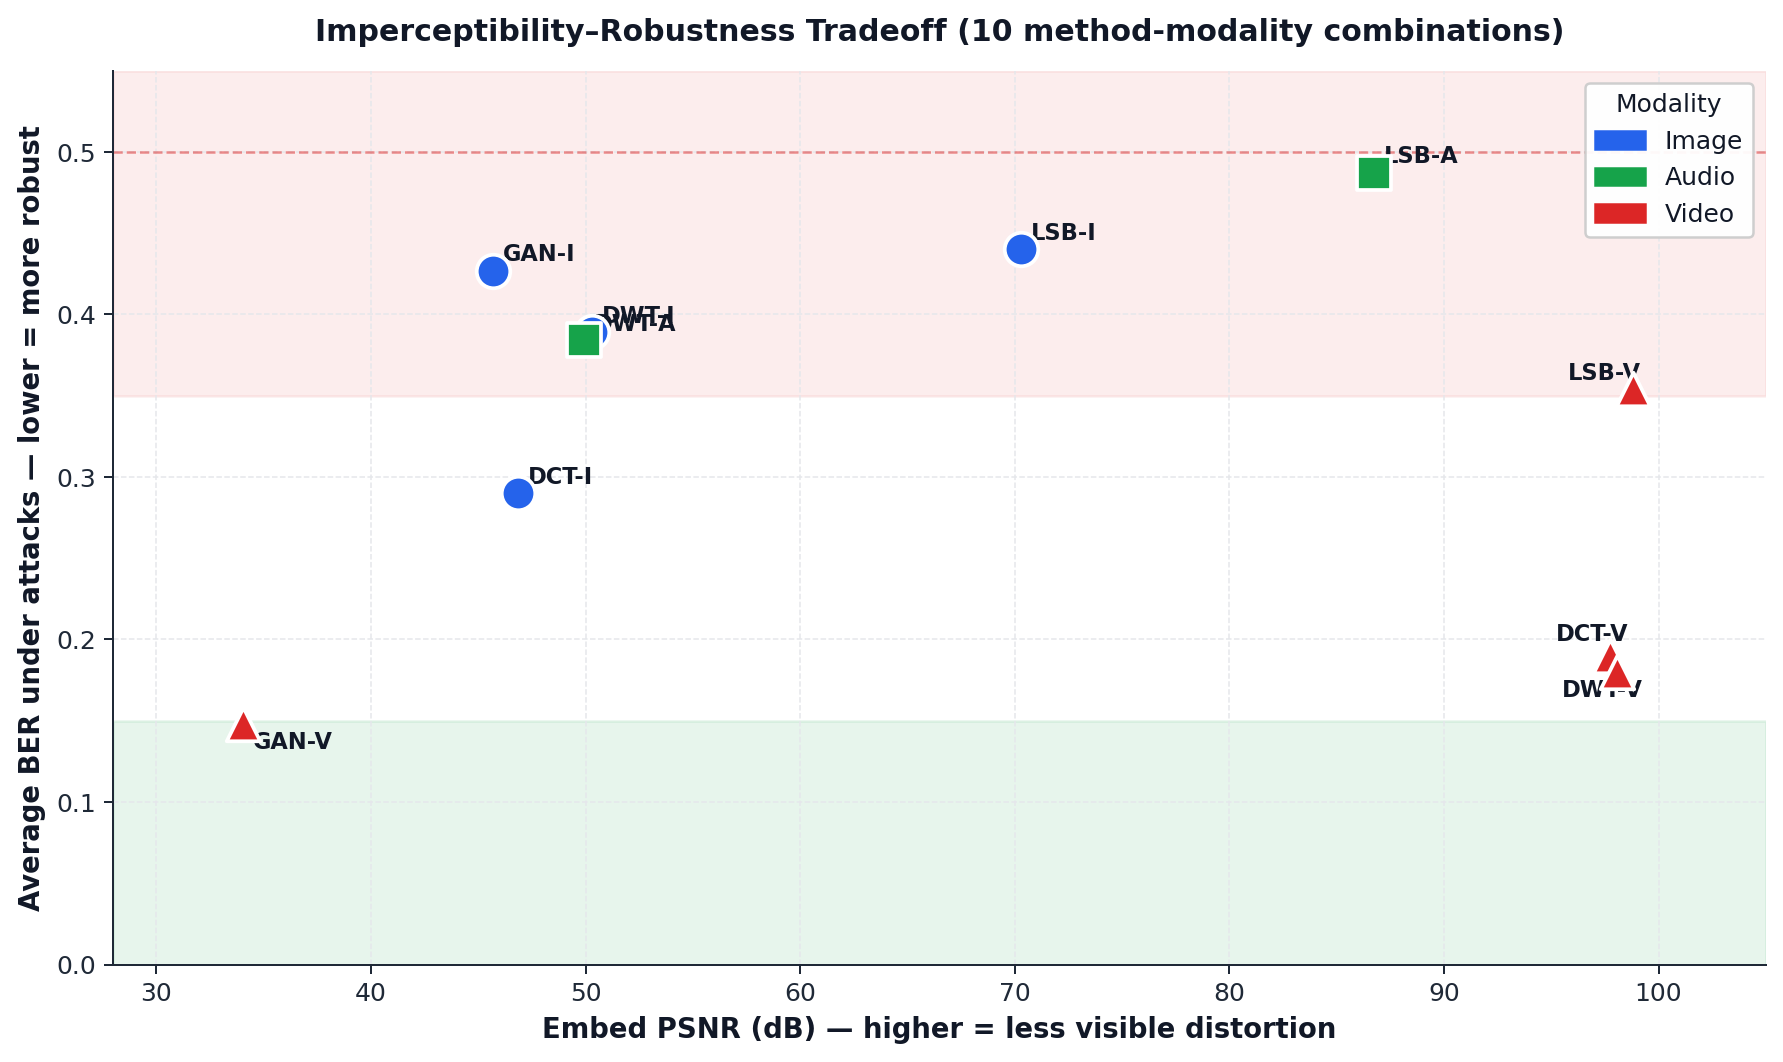
\includegraphics[width=\columnwidth]{chart_psnr_tradeoff.png}}
\caption{Imperceptibility–robustness tradeoff for all eight
method-modality combinations. Higher embed PSNR = less visible change;
lower BER = more robust. Green shaded region: robust zone (BER $<
0.15$); red shaded region: fragile zone (BER $\geq 0.35$). The video
GAN alone falls in the robust zone.}
\label{fig_tradeoff}
\end{figure}

Three distinct clusters emerge from Fig.~\ref{fig_tradeoff}.

\textit{Cluster 1 — High PSNR, Fragile (top-right):} LSB across both
modalities groups here with embed PSNR ranging from 70.27~dB
(image) to 98.79~dB (video) but average BER between 0.354 and 0.440,
placing all LSB configurations firmly in the fragile zone. This is the
canonical imperceptibility-without-robustness profile of spatial-domain
methods: minimal signal modification yields high quality, but that
modification resides in the exact signal layer—the least significant
bits—most vulnerable to any subsequent processing.

\textit{Cluster 2 — Moderate PSNR, Moderate Robustness (middle):}
DCT and DWT for both image and video cluster here, with embed PSNR
between 46--50~dB and average BER between 0.180 and 0.427. Transform-domain
embedding accepts a reduction in PSNR (embedding in perceptually
significant but attack-resistant frequency components) in exchange for
meaningful robustness gains. The best result in this cluster—DWT video
at BER 0.180—is 49\% lower BER than LSB video (0.354) at a cost of
only 0.74~dB in embed PSNR.

\textit{Cluster 3 — Low PSNR, Robust (bottom-left):} The video GAN
sits in isolation here with embed PSNR of 34.03~dB and BER of 0.148.
No other configuration achieves BER below 0.15 (the robust threshold).
The GAN encoder's learned strategy modifies a broader set of
spatiotemporal coefficients to distribute the message redundantly
across attack-resistant signal features, accepting greater visible
distortion as the necessary cost.

The tradeoff plot confirms the fundamental prediction of steganography
theory: no single method simultaneously achieves high
imperceptibility and high robustness. Each point in the plot represents
a different position on the Pareto frontier between these two
objectives. The appropriate operating point depends on the deployment
scenario:

\begin{itemize}
    \item Use \textbf{LSB} when the carrier is stored and transmitted
    losslessly and maximum perceptual quality is mandatory.
    \item Use \textbf{DCT} when JPEG or H.264 frame compression is
    the dominant expected attack on image or video carriers.
    \item Use \textbf{DWT} when diverse attack types are expected and
    a balanced tradeoff is required across image or video.
    \item Use \textbf{GAN} for video transmission over lossy or
    adversarial channels where maximum robustness is the priority
    and a 34~dB embed PSNR is acceptable.
\end{itemize}

% ─────────────────────────────────────────────────────────────────────────────
\section{Steganalysis Resistance}
% ─────────────────────────────────────────────────────────────────────────────

Beyond robustness against signal processing attacks, a practical
steganographic system must resist detection by an adversary performing
statistical analysis on the carrier. We discuss the detectability
profile of each method qualitatively.

\textbf{LSB.} LSB substitution is well-known to be detectable by
statistical analysis. The most prominent attack is the
Chi-Square~($\chi^2$) test: natural images exhibit a
specific statistical relationship between pairs of pixel values that
differ only in their LSB; LSB embedding disrupts this relationship,
producing a characteristic signature. Sample Pairs (SP) analysis and
Rich Model (SRM) steganalysts can detect LSB embedding with high
accuracy even at low embedding rates, as evaluated extensively in
recent steganalysis robustness studies \cite{b6}.

\textbf{DCT and DWT.} Transform-domain methods are substantially
harder to detect than LSB because they modify frequency coefficients
rather than raw pixel values. The coefficient histograms of DCT-stego
images are less distinguishable from those of cover images than LSB
histograms. However, blind steganalysts trained on large image
databases \cite{b6} can still achieve meaningful detection rates
against DCT and DWT methods at moderate embedding rates.

\textbf{GAN.} The GAN method is the hardest to detect statistically.
The discriminator during training directly minimises the statistical
distance between the cover and stego distributions, explicitly
penalising any detectable deviation \cite{b11}. This adversarial
training produces stego images that resist histogram and
frequency-domain analysis more effectively than classical methods.
Dedicated GAN-stego detectors \cite{b12} have been proposed but
require specific training against the target GAN architecture;
general-purpose steganalysts are not reliably effective against
GAN-based embedding. This makes the GAN method the strongest choice
not only for robustness but also for resistance to automated
steganalysis.

% ─────────────────────────────────────────────────────────────────────────────
\newpage
\section{Conclusion}
% ─────────────────────────────────────────────────────────────────────────────

This paper presented a unified multi-modal steganography system
integrating LSB, DCT, DWT, and GAN embedding across image and
video carriers, secured with AES-256-GCM authenticated encryption and
Reed-Solomon error correction for classical methods. The system is
fully deployed as a containerised web application. A comprehensive
evaluation framework covering 22 attack configurations across two
media types provides quantitative evidence for method selection in
practical deployment scenarios.

The evaluation reveals a clear performance hierarchy. The video GAN
achieves the highest overall robustness with average BER of 0.148—the
only method in the defined Robust zone (BER $< 0.15$)—owing to the
H.264 codec noise layer used during training. DCT provides the best
classical robustness for images (avg BER 0.290) and video (avg BER
0.190), consistently surviving JPEG compression with BER $= 0.000$
at Q=90 and Q=75. LSB, despite providing the highest embedding quality
(70--99~dB PSNR), is classified Fragile or Moderate across all
configurations. The imperceptibility–robustness tradeoff confirms that
no single method simultaneously maximises both objectives: each
configuration represents a distinct operating point on the Pareto
frontier.

\textit{Limitations and Future Work.} The CPU-only training constraint
limited GAN spatial resolution to 64$\times$64 pixels, and the image
GAN was trained without a JPEG-specific noise layer, limiting its
still-image compression robustness. Planned extensions include GPU
retraining at 128$\times$128 resolution, JPEG noise layer integration
in the image GAN pipeline, and formal steganalysis evaluation
against modern detectors \cite{b6}, \cite{b12}.


% ─────────────────────────────────────────────────────────────────────────────
\begin{thebibliography}{00}

\bibitem{b1}
D. Yang, J. Yu, H. Wang, W. Wang, C. Weng, Y. Zou, D. Yu, J. Xi,
Z. Xia, W. Zhang, Y. Xie, and L. Zhao,
``Diffusion-based model for audio steganography,''
\textit{Electronics}, vol.~14, no.~20, art.~no.~4019, Oct.~2025.

\bibitem{b2}
K. R. Malik, M. Sajid, A. Almogren, T. S. Malik, A. H. Khan,
A. Altameem, A. Ur Rehman, and S. Hussen,
``A hybrid steganography framework using DCT and GAN for secure data
communication in the big data era,''
\textit{Scientific Reports}, vol.~15, art.~no.~19620, Jun.~2025.

\bibitem{b3}
C. Han and T. Xue,
``Adaptive network steganography using deep learning and multimedia
video analysis for enhanced security and fidelity,''
\textit{PLoS ONE}, vol.~20, no.~6, art.~no.~e0318795, Jun.~2025.

\bibitem{b4}
C.-C. Chang and I. Echizen,
``Steganography beyond space-time with a chain of multimodal AI,''
\textit{Scientific Reports}, vol.~15, art.~no.~12908, Apr.~2025.

\bibitem{b5}
Y. Sanjalawe, S. R. Al-Emari, S. Fraihat, and M. Abualhaj,
``A deep learning-driven multi-layered steganographic approach for
enhanced data security,''
\textit{Scientific Reports}, vol.~15, art.~no.~4761, Feb.~2025.

\bibitem{b6}
O. A. AlRusaini,
``Deep learning for steganalysis: Evaluating model robustness against
image transformations,''
\textit{Frontiers in Artificial Intelligence}, vol.~8,
art.~no.~1532895, 2025.

\bibitem{b7}
X. Li, Y. Zhang, K. Liao, W. Li, and X. Li,
``EStegTGANs: Enhanced steganography based on transform domain GAN,''
\textit{Multimedia Systems}, vol.~30, no.~3, pp.~1--15, 2024.

\bibitem{b8}
J. Zhu, R. Kaplan, J. Johnson, and L. Fei-Fei,
``HiDDeN: Hiding data with deep networks,''
in \textit{Proc. European Conf. Computer Vision (ECCV)},
2018, pp.~657--672.

\bibitem{b9}
M. Hussain, A. W. A. Wahab, Y. I. B. Idris, A. T. S. Ho, and K.-H. Jung,
``Image steganography in spatial domain: A survey,''
\textit{Signal Process.: Image Commun.}, vol.~65, pp.~46--66, Jul.~2018.

\bibitem{b10}
S. Baluja,
``Hiding images in plain sight: Deep steganography,''
in \textit{Proc. Advances in Neural Information Processing Systems
(NIPS)}, 2017, pp.~2066--2076.

\bibitem{b11}
D. Volkhonskiy, I. Nazarov, B. Borisenko, and E. Burnaev,
``Steganographic generative adversarial networks,''
\textit{arXiv preprint arXiv:1703.05502}, 2017.

\bibitem{b12}
M. Xu, G. Li, Z. Wang, P. Zhang, A. Jiang, and Y. Guo,
``Structural design of convolutional neural networks for steganalysis,''
\textit{IEEE Signal Process. Lett.}, vol.~23, no.~5,
pp.~708--712, May~2016.

\end{thebibliography}

\end{document}
